%\begin{figure}[H]
%	\begin{center}
%		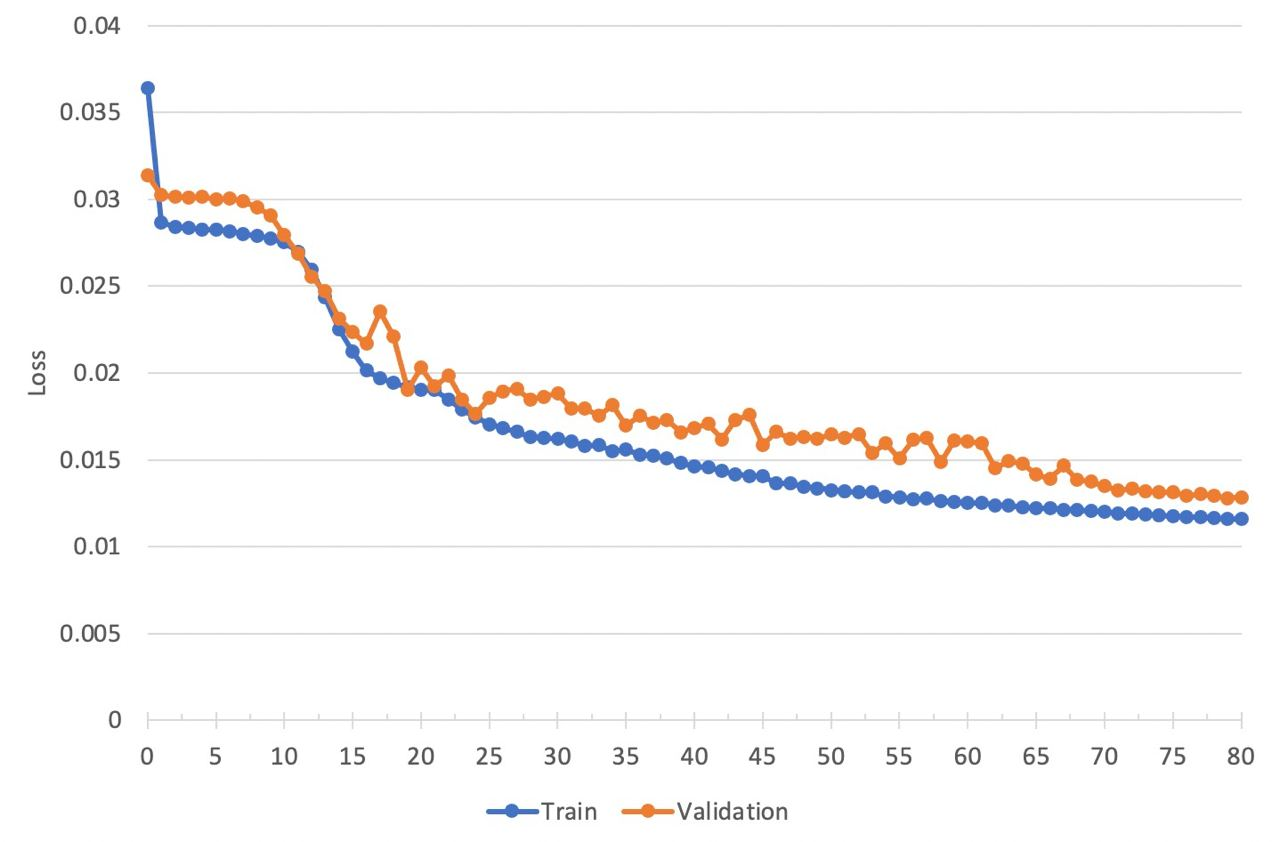
\includegraphics[width=0.5\linewidth]{bilder/nuclei/no-wi.jpg}
%		\caption{Default weight initialization is not suitable}\label{fig:no-wi}
%	\end{center}
%\end{figure}

%\begin{figure}[H]
%	\begin{center}
%		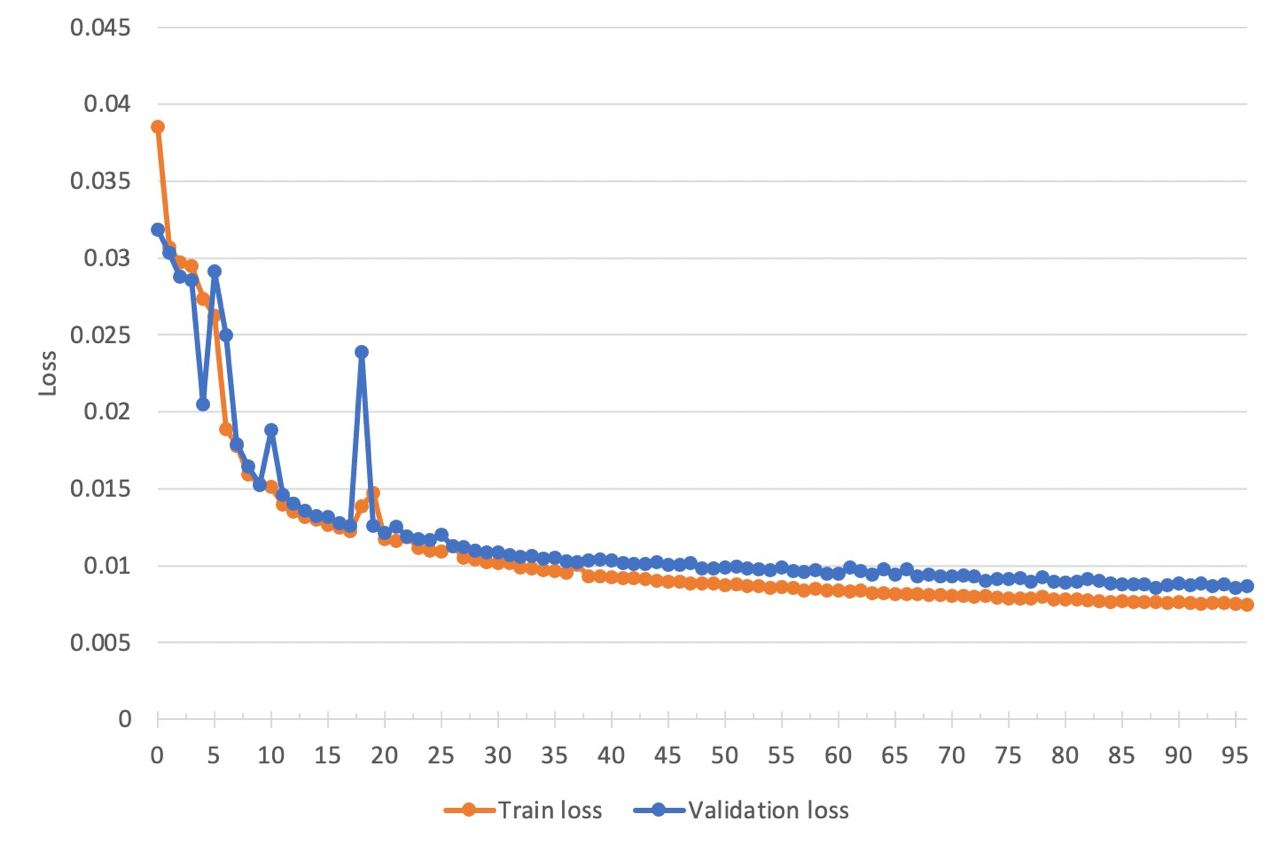
\includegraphics[width=0.5\linewidth]{bilder/nuclei/pca-2-datasets.jpg}
%		\caption{PCC with correct weight initialization converges but unstable}\label{fig:pcc-2-dataset}
%	\end{center}
%\end{figure}

\begin{figure}[H]
	\begin{center}
		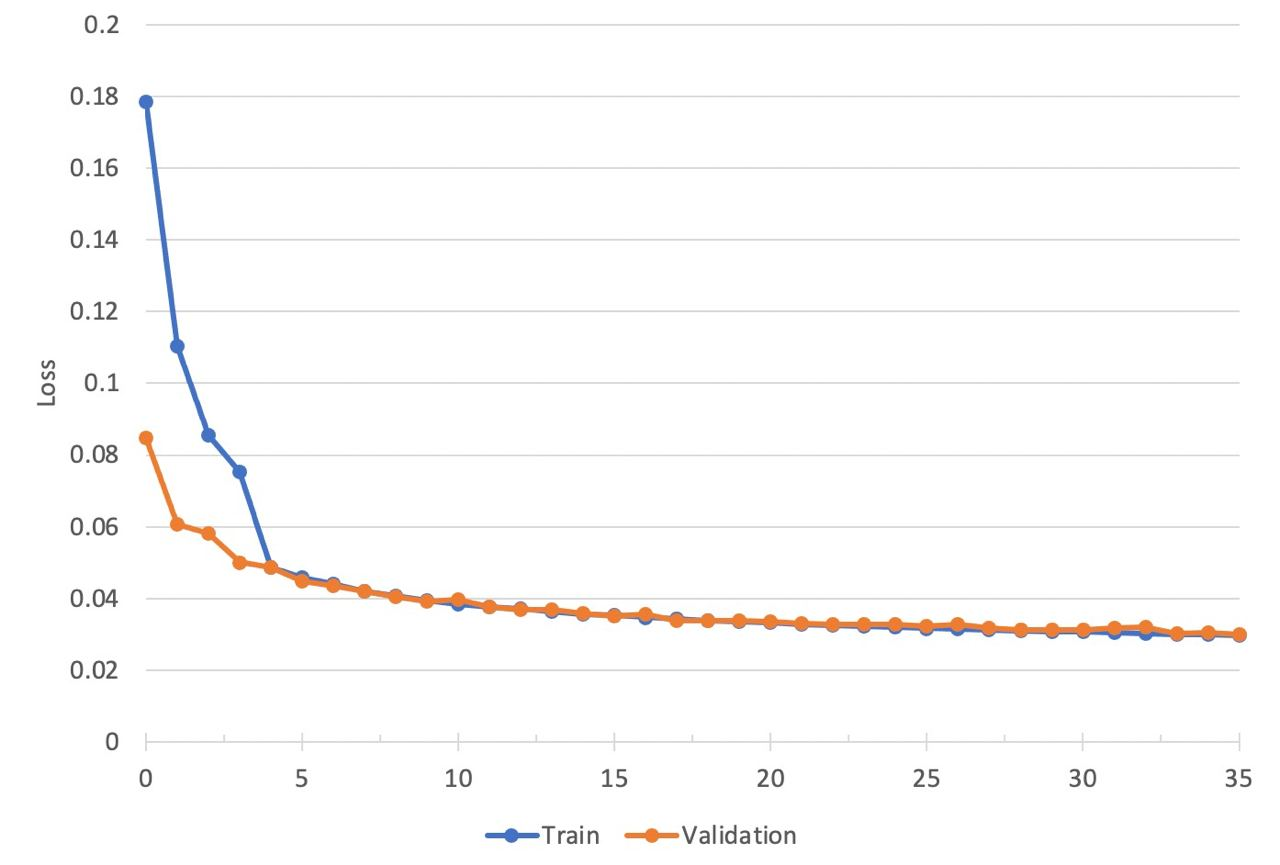
\includegraphics[width=0.5\linewidth]{bilder/nuclei/full-dataset.jpg}
		\caption{Having more data makes training more stable}\label{fig:full-dataset-pcc}
	\end{center}
\end{figure}

\begin{figure}[H]
	\begin{center}
		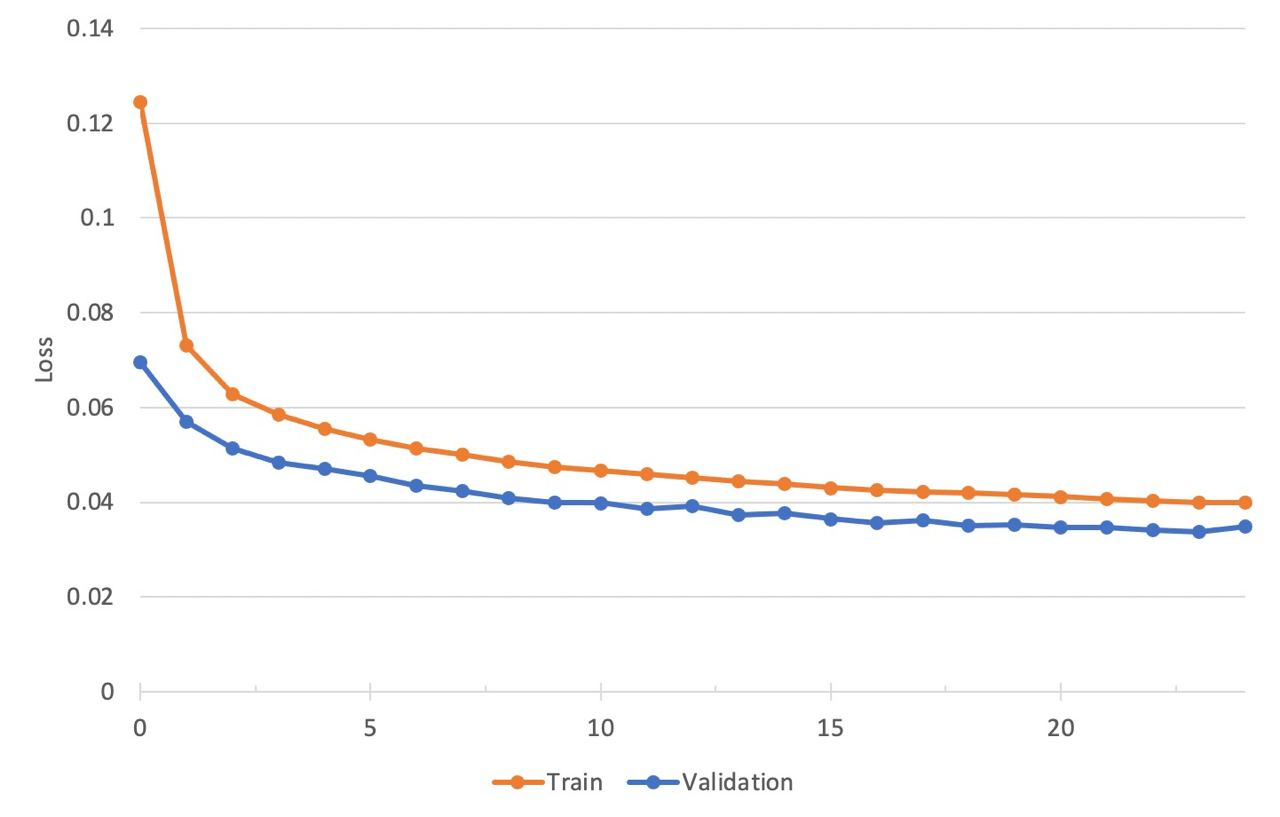
\includegraphics[width=0.5\linewidth]{bilder/nuclei/full-dataset-regularized.jpg}
		\caption{With regularization and augmentations PCC}\label{fig:full-dataset-pcc-regularized}
	\end{center}
\end{figure}

\begin{figure}[H]
	\begin{center}
		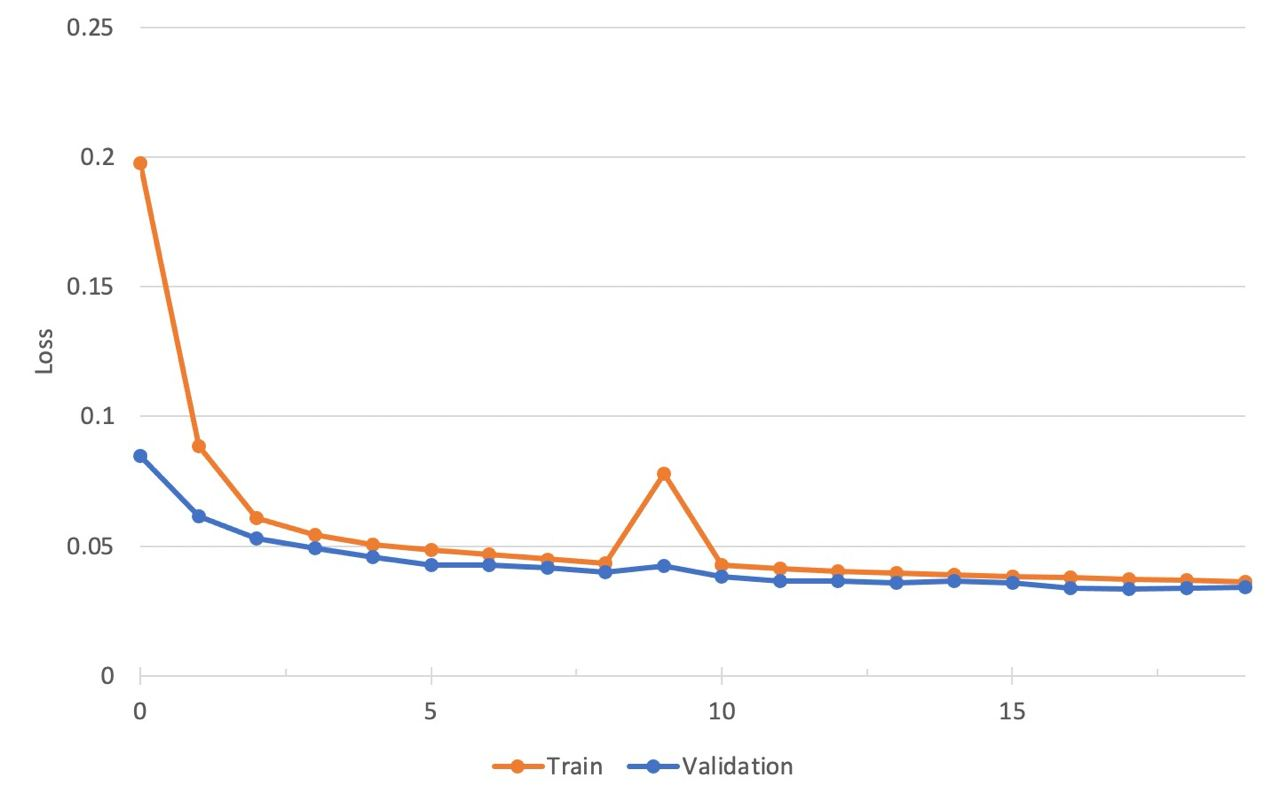
\includegraphics[width=0.5\linewidth]{bilder/nuclei/no-reg-but-aug.jpg}
		\caption{No regularization but augmentations}\label{fig:no-reg-augmented}
	\end{center}
\end{figure}

\begin{figure}[H]
	\begin{center}
		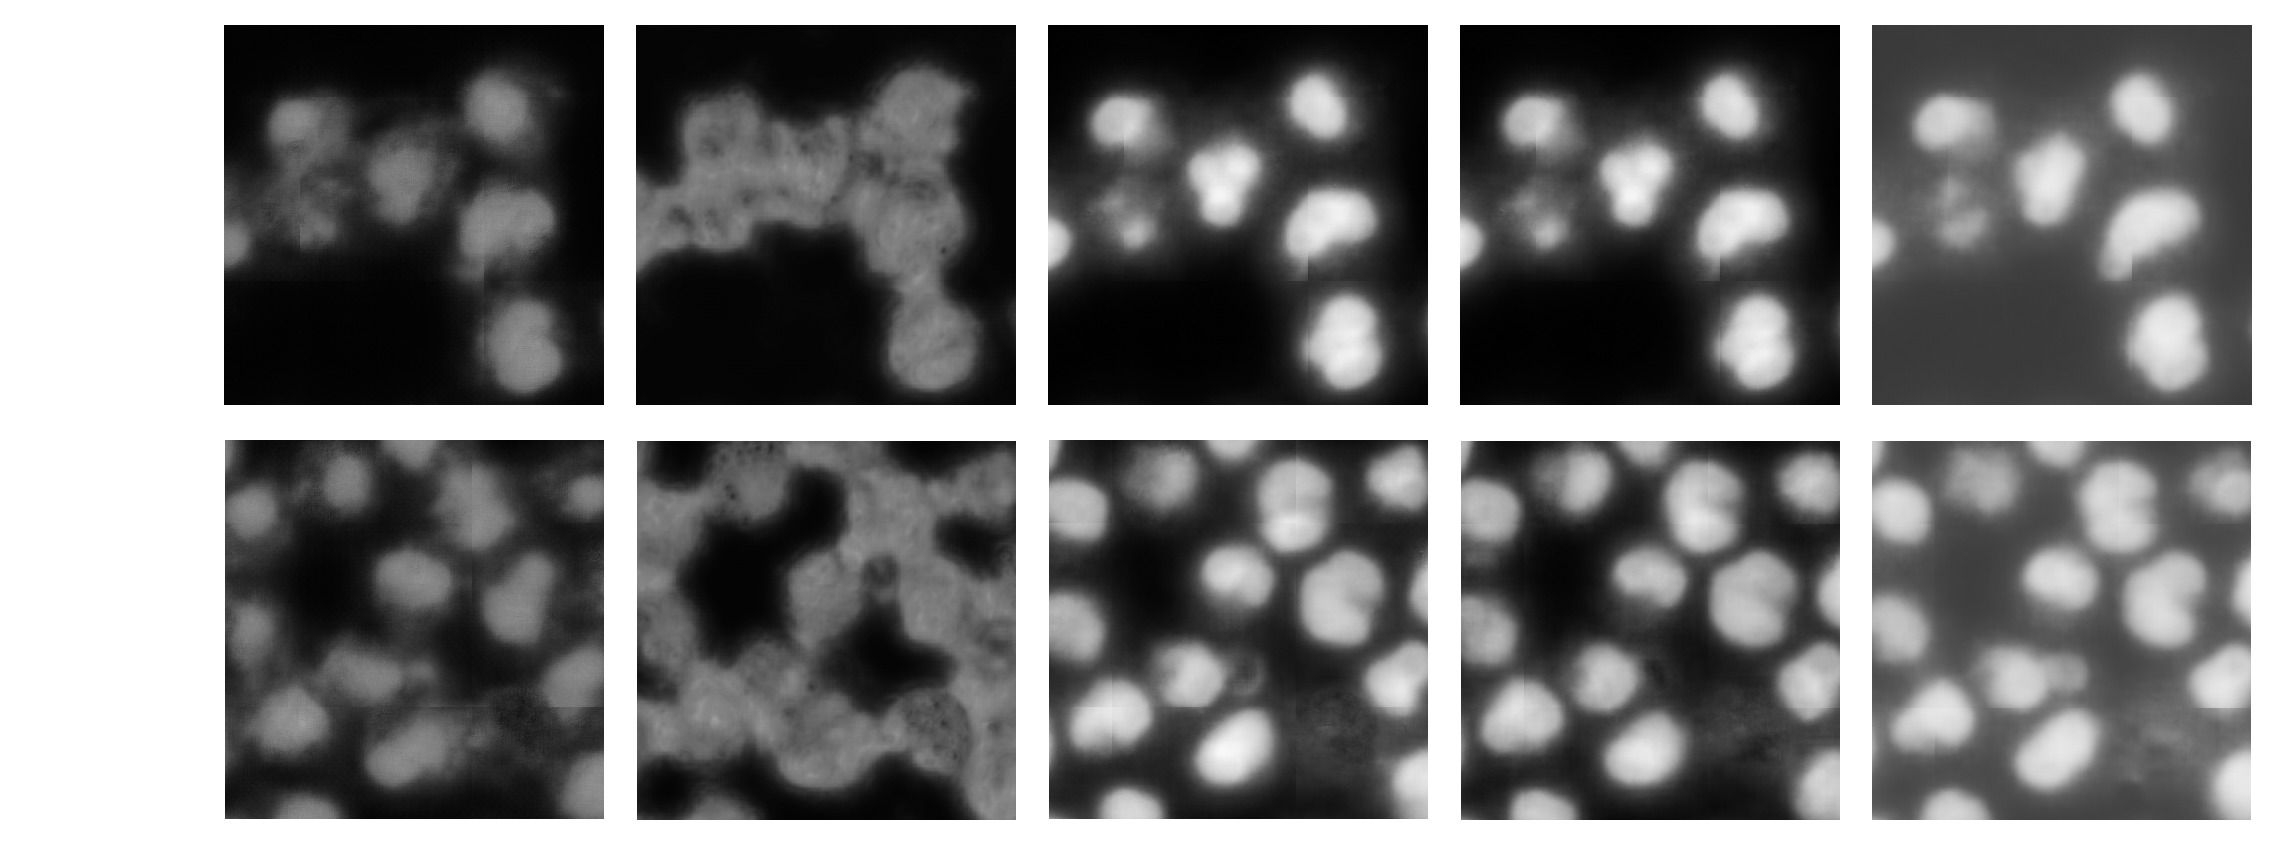
\includegraphics[width=0.5\linewidth]{bilder/nuclei/comparison-chzn-phx.png}
		\caption{Difefrent models predictions and scores comparison}\label{fig:nuclei-comparison-predictions}
	\end{center}
\end{figure}